\section{图表公式}
\subsection{公式}\label{sec:eq}
见公式 \ref{eq:mc2}。
\begin{equation}\label{eq:mc2}
E = m c^2
\end{equation}
\subsection{图}\label{sec:fig}
问题二结果见图\ref{fig:prob1}。
\begin{figure}[!htb]
\centering
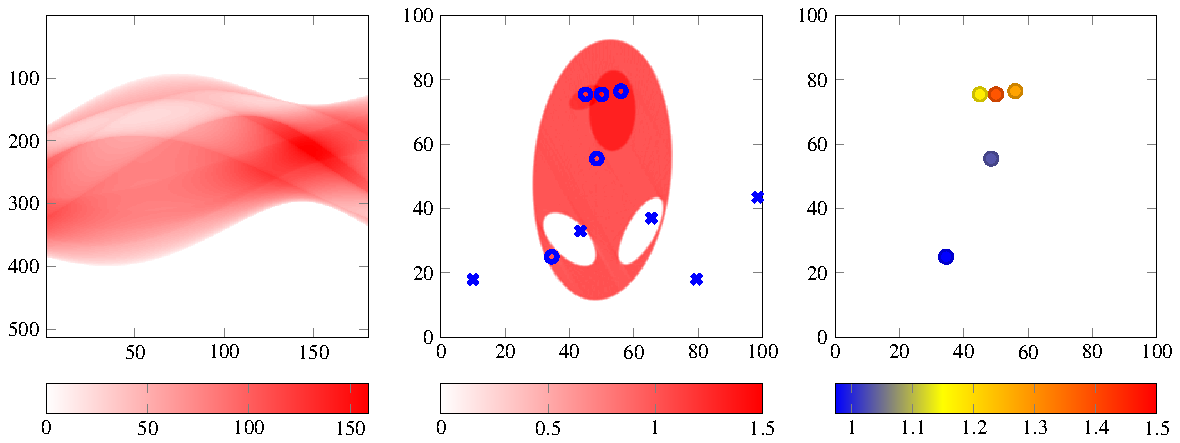
\includegraphics[width=\textwidth]{fig}
\caption{问题二结果图}\label{fig:prob1}
\end{figure}

\subsection{表}
表格应具有三线表格式,如表 \ref{tab:three} 所示。
\begin{table}[!htb]
\caption{标准三线表格}\label{tab:three} \centering
\begin{tabular}{ccccc}
\toprule[1.5pt]
$D$(in) & $P_u$(lbs) & $u_u$(in) & $\beta$ & $G_f$(psi.in)\\
\midrule[1pt]
 5 & 269.8 & 0.000674 & 1.79 & 0.04089\\
10 & 421.0 & 0.001035 & 3.59 & 0.04089\\
20 & 640.2 & 0.001565 & 7.18 & 0.04089\\
\bottomrule[1.5pt]
\end{tabular}
\end{table}

\subsection{引用}
第\ref{sec:eq}小节给出了一个公式的例子。第一问的解题程序见附录 \ref{sec:cod} 中的代码 \ref{cod:getparm}。随便胡乱的引一个文献 \cite{Beauregard2005},再引两个 \cite{Hicks2006,王永庆1998}。
